\documentclass[a4paper,12pt]{article}


%%%%%%%%%%%%%%%%%%%%%%%%%%%%%% BEGIN-Packages %%%%%%%%%%%%%%%%%%%%%%%%%%%%%
\usepackage{amsmath,amssymb,amsfonts}
\usepackage{mathrsfs,enumerate}
\usepackage{color,xcolor}
\usepackage{graphicx,subfigure}
\usepackage{clock} % Use this package to insert a clock in the beamer.
\usepackage{textcomp}
\usepackage[T1]{fontenc}
\usepackage{verbatim}
\usepackage{moreverb}
\usepackage{booktabs}
\usepackage{tabularx}
\usepackage{multirow,multicol}
\usepackage{natbib}
\usepackage[ruled,lined,linesnumbered]{algorithm2e}
%\usepackage{algorithm2e}
%\usepackage{url}
%\usepackage{hyperref}
\usepackage[colorlinks,linkcolor=black,citecolor=black,urlcolor=black]{hyperref}%[colorlinks,linkcolor=blue,citecolor=blue,urlcolor=blue]
\usepackage{CJK}
%%%%%%%%%%%%%%%%%%%%%%%%%%%%%%%% END-Packages %%%%%%%%%%%%%%%%%%%%%%%%%%%%%


% \setbeamertemplate{navigation symbols}{} % Disable the buttons at the bottom.

\graphicspath{{Figures/}} % Set the directory where figures are saved.

%%%%%%%%%%%%%%%%%%%% BEGIN-Theorem-like Environments %%%%%%%%%%%%%%%%%%%%%
%\newtheorem{mybox}{}
\newtheorem{Con}{Conjecture}[section]
\newtheorem{Thm}{Theorem}[section]
\newtheorem{Prop}{Proposition}[Thm]
%%%%%%%%%%%%%%%%%%%%% END-Theorem-like Environments %%%%%%%%%%%%%%%%%%%%%%


%%%%%%%%%%%%%%%%%%%%%%%%%% BEGIN-New Commands %%%%%%%%%%%%%%%%%%%%%%%%%%%%
\newcommand{\email}[1]{\href{mailto: #1}{\tt {\color{blue}#1}}}
\newcommand{\red}{\color{red}}
\newcommand{\blue}{\color{blue}}
\newcommand{\green}{\color{green}}
\newcommand{\brown}{\color{brown}}
\newcommand{\orange}{\color{orange}}
\newcommand{\yellow}{\color{yellow}}
\newcommand{\white}{\color{white}}
\newcommand{\Real}{\mathbb{R}}
\newcommand{\Tran}[1]{#1^\mathrm{T}}
\newcommand{\st}{\textnormal{s.t.}}
\newcommand{\dist}{\textnormal{dist}}
\newcommand{\bc}{\begin{center}}
\newcommand{\ec}{\end{center}}
\newcommand{\bl}{\begin{flushleft}}
\newcommand{\el}{\end{flushleft}}
\newcommand{\tbf}{\textbf}
\newcommand{\be}{\begin{equation}}
\newcommand{\ee}{\end{equation}}
\newcommand{\ba}{\begin{array}}
\newcommand{\ea}{\end{array}}
\newcommand{\btab}{\begin{table}\begin{tabular}}
\newcommand{\etab}{\end{tabular}\end{table}}
\newcommand{\nn}{\nonumber}
\newcommand{\xn}{x_1,x_2,\ldots,x_n}
\newcommand{\framee}[2]{\frame{\frametitle{#1} #2}}
\newcommand{\reff}[1]{(\ref{#1})} % 免得敲()
\newcommand{\inner}[2]{\left\langle#1,#2\right\rangle}
\newcommand{\paper}[1]{({\blue \footnotesize{#1}})}
\newcommand{\hd}[1]{\multicolumn{1}{c}{#1}}


\newcommand{\rmnum}[1]{\romannumeral #1}
\newcommand{\Rmnum}[1]{\expandafter\@slowromancap\romannumeral #1@}
%%%%%%%%%%%%%%%%%%%%%%%%%%%% END-New Commands %%%%%%%%%%%%%%%%%%%%%%%%%%%%


\begin{document}
\title{Geometric buildup-based error minimization algorithms for protein structure determination problems with sparse large-noisy distances}
\author{Zhenli Sheng, Yaxiang Yuan}
\date{\today}
\maketitle

\noindent \textbf{Abstract~}  Distance Geometry Problem has attracted a great deal attentions in recent years due to its wide applications in biology, environmental monitor and sensor-based applications, etc. Based on the fast Geometric Buildup algorithms developed by Wu and his coauthors \cite{Dong2003,Wu2008,Sit2009}, we propose enhanced Geometric Buildup algorithms (GBEM-LLS and GBEM-NLS). Our main contribution is two-fold. First, we analysis the importance of computation order and carefully design a buildup sequence to make our algorithms much more stable than before. Second, an novel framework is proposed such that error minimization technique is integrated in every buildup process to control error accumulation effectively, which is a dominant disadvantage of the original algorithms. Extensive numerical experiments show that our algorithms can give reasonably good results in short computation time. For instance, given inter-atomic distances which are less than $6$\AA ~and are corrupted with $10\%$ multiplicative noise, a 5681-atom can be realized within $3$ minutes with a root-mean-square-deviation (RMSD) of $0.24$\AA. The former state-of-the-art Geometric Buildup methods \cite{Sit2009} can only handle at most $0.01\%$ noise with distances under $6$\AA, our novel algorithms can deal with $10\%$ noises, which makes the Geometric Buildup methods practical, hence can be applied in real problems.

\section{Introduction}
There exist many ways to describe \emph{Distance Geometry Problem} (henceforth, DGP), we favor the graph language as following,

%\noindent \framebox{\parbox{0.98\textwidth}{
For a graph $G=(V,E)$, where $V$ is the vertex set and $E$ is the edge set, given some distances $d_{ij},$ for $(i,j) \in E$, the aim is to find $x_1, x_2, \ldots, x_n \in \Real^d$ (where $d$ is prescribed), such that
\be \|x_i-x_j\| = d_{ij}, ~~ (i,j) \in E. \ee
%}}

In the ideal case, no errors exist in the distance $d_{ij}$, the problem is called \emph{DGP with exact (noiseless) distances}, otherwise it is called \emph{DGP with inexact (noisy) distances}. In an even more realistic case, rather than the distance $d_{ij}$, but the upper bound $u_{ij}$ and lower bound $l_{ij}$ are given for each edge in $E$, then we need to find coordinates $x_i \in \Real^d$ satisfying the following inequalities instead,
\be l_{ij} \leq \|x_i-x_j\| \leq u_{ij}, ~~ (i,j) \in E. \ee
Problem in this version is called \emph{DGP with distance bounds}. In the rest of this paper, we focus on \emph{DGP with noisy distances}.

\emph{DGP with exact distances} has been proved to be NP-hard in general \cite{Saxe1979}, a proof the corresponding noisy case can be found in \cite{Wu2008}. Therefore, it is impossible to find polynomial-time algorithms to solve all the instances of this problem unless $P=NP$, though some special instances like \emph{K-trilateration graph} \cite{Maculan2014} do admit polynomial-time approach.

This mathematical problem has a large number of applications in different fields, here we just list a few of them. In graph drawing area \cite{Gansner2005}, it is called \emph{Graph Realization Problem}, in which the task is to draw a graph such that the distances between points reveal the given weights.  
In this paper, we study an important application in computational biology, which is called \emph{Protein Structure Determination} \cite{Braun1987,Sit2011,Voller2013}, in some literatures, it is also called \emph{Molecular Conformation Problem} \cite{Crippen1988,Biswas2008,Fang2013} or \emph{Molecular Distance Geometry Problem} \cite{Dong2002,Dong2003,Carvalho2008}. In this problem, a part of the pairwise distances between atoms either can be measured by Nuclear Magnetic Resonance (NMR) or X-ray Crystallography technique, or can be estimated based on biological information, such as bond angle and bond length. Many properties of proteins are heavily relied on the three-dimensional structure of the proteins, which makes the determination of the relative coordinates of the atoms so important (the distance remains the same if the whole structure is moved under rigid transformations including translations, rotations and reflections, this is why we call the locations are relative coordinates).

Another important application is called \emph{Wireless Sensor Network Localization} \cite{Akyildiz2002,Chong2003,Mao2007,Yick2008}. Sensor is an efficient tool for environmental monitoring, animal management, and even in military operations, since it is cheap and convenient. Usually every unit is equipped with a sensor, which can send radio signals, collect and process simple information. Determining the location of the sensors usually is the first step because many further applications are location-related. The sensors can send signals within some radio range, thus the distance of nearby sensors can be measured by the difference of arrival time or the decay of the signal, the latter is more accurate in general. A main feature of this application differing from others is that the exact location of a small portion of the sensors are known in advance, those are called \emph{anchors}.

Notice that the distances in the last two applications both are local due to the limitation of the NMR techniques or the power of the sensors, which means only distances within some cutoff range are known. As a result, the distance information is very sparse as a whole, that is to say, the known distances is only a small portion of all the pairwise distances.

In the rest of this paper, we focus on the protein structure determination, that is to say, we consider the three-dimensional anchor-free DGP and the points are atoms. We first model the problem as an optimization problem in Section \ref{sec:errfun}, then review some related works in Section \ref{sec:related}. A somehow detailed review on the original Geometric Buildup methods is presented in Subsection \ref{subsec:GB}. Following that we give the framework and details of our algorithm in Section \ref{sec:alg}. Problem setting and extensive numerical results are provided in Section \ref{sec:num}. Further discussions and possible extensions are given in Section \ref{sec:extension}.

\textbf{Notations} Throughout this paper, vectors are column vectors and are denoted by lower-case letters, matrices are denoted by capital letters. For a vector $x\in \Real^n$, $\|x\|=\sqrt{x^Tx}$ is the Euclidean 2-norm, for a matrix $X\in \Real^{m\times n}$, $\|X\|_F=\sqrt{tr(X^TX)}$ is the Frobenius norm. $A=(a_{ij})$ means that the elements in matrix $A$ are $a_{ij}$. $A(:,1:k)$ denotes the 1 to $k$ columns of $A$ in a Matlab fashion, $A(1:k,1:k)$ is the upper left $k$-dimensional submatrix. $e_i$ is the $i$-th column of the identity matrix. We use subscript $i$ to denote the $i$-th component of a vector, and superscript $k$ to denote the iteration number. Conformation, configuration, layout and location are used interchangeably to denote the coordinates of all the atoms in a certain protein.

\section{Error Minimization Models}\label{sec:errfun}
We have introduced DGP as a feasible problem of a collection of equations, but it is usually solved by modeling as an unconstrained optimization problem,
\be \min_{\xn} f(\xn), \label{prob:error}\ee
where $x_i$ are the coordinates of the points, $f(\cdot)$ is an error function which measures the deviations between computed distances and given ones. In the literatures, the most commonly used error functions for DGP are as follows,
\begin{itemize}
  \item Stress function
  \be Stress(\xn) = \sum_{(i,j)\in E} \omega_{ij}(\|x_i-x_j\|-d_{ij})^{2}, \label{eqn:stress}\ee
  \item Smoothed Stress function
  \be SStress(\xn) = \sum_{(i,j)\in E} \omega_{ij}(\|x_i-x_j\|^2-d_{ij}^2)^{2},\label{eqn:sstress}\ee
  \item Absolute Error function
  \be AbsErr(\xn) = \sum_{(i,j)\in E} \omega_{ij}\left|\|x_i-x_j\|^2-d_{ij}^2
   \right|, \label{eqn:abserr}\ee
\end{itemize}
where $\omega_{ij}$ are the weights on edges, which can be chosen properly to generate suitable models. For example, we choose all $\omega_{ij}$ to be 1 to treat all the distance data equally, or we can set it small if we do not trust a certain data or set it large to emphasis a certain data. One special choice is $\omega_{ij}=1/d_{ij}^2$ in \reff{eqn:stress}, thus the model measures the relative errors instead.

Among them, $AbsErr$ is usually used by SDP-based models as described in Subsection \ref{subsec:sdp}. Rather than $Stress$, the gradient of $SStress$ is continuous since the norm term---$\|x_i-x_j\|$ does not show up in the denominator, which is what earns this function its name.
%Therefore, in this paper, we choose $SStress$ as our error function.

It is easy to observe that, if the given distances are exact, finding the true coordinates is equivalent to finding the global solution of these error functions, whose function value is zero. However, all the error functions have extremely large number of local minimizers \cite{Nocedal1999} (Page 14), and most of the local minimizers are meaningless to us, which makes the problem so challenging because conventional continuous optimization techniques like gradient descent or Newton's method can only guaranty to find a stationary point or a local minimizer. Consequently, it is necessary to take advantage of some other methods like SDP relaxation to obtain a coarse layout and minimize an error function to further improve the result \cite{Biswas2008,Fang2013}. These papers emphasis the SDP process and use error minimization as a postprocess procedure. The optimization method to minimize error functions are somehow standard, thus the authors usually do not say much about it, which gives us an impression that this process is useful but do not stand at the center of the algorithm. However, we would like to view these techniques as a way to obtain a good initial point to accomplish our final task---finding the global or at least a good approximate solution to the error functions, that is to say, we emphasis the optimization procedure and view other techniques as auxiliary methods. Actually, this point of view gives us the motivation to introduce error function minimization procedure to every buildup step and finally achieve significant improvement, the details will become clear later.

We emphasis again that since we do not have anchor points, the whole configuration remains the same under rigid transformations, what we get from the algorithms are just the relative coordinates up to any rigid transformations.

%that is why we need the buildup process to find a good initial layout. If the buildup process is successful, gradient descent method is enough to find a nearby minimizer, while second-order method is too expensive for calculation.
 
\section{Related works}\label{sec:related}
The prior works about this problem trace back to \cite{Schoenberg1935} in 1935 and \cite{Blumenthal1953,Torgerson1958}. After that, a large amount of algorithms have been proposed and each of them has its own pros and cons. We review some of them for our own interest in this section but have no attempt to cover them all. For example, we do not give the details of \cite{Qi2012}, which is also an interesting paper working on the rank constrained reduced distance matrix, based on an old result in \cite{Schoenberg1935}. For a brief summary of existing methods, see Table 13.1 in \cite{Fang2013}. For those who have further interests, we refer them to \cite{Maculan2014}, which is a recently published exhaustive survey paper in SIAM Review.

\subsection{Matrix Decomposition Method}\label{subsec:MatDcomp}
In \cite{Blumenthal1953}, a matrix decomposition method is proposed to solve the DGP with full set of distances, by full set we mean all the pairwise distances are known. It is the oldest mature method for DGP to our knowledge, but is still very important because it is the foundation of many other methods. We give the details of this algorithm as below due to its fundamental position and its usage in our algorithms.

Since the whole structure is invariant under rigid transformations, without lose of generality, we set $x_n$ at origin, i.e., $x_n = (0,0,0)^T$. Then we have $d_{in} = \|x_i-x_n\| = \|x_i\|$. Moreover, by taking the square of both sides of $\|x_i-x_j\| = d_{ij}$, we obtain
\be \|x_i\|^2 - 2x_i^Tx_j + \|x_j\|^2 = d_{ij}^2, ~~\textrm{for } i,j = 1,2,\ldots,n-1.\ee
By substituting $\|x_i\|$ with $d_{in}$, and moving known items to one side, we have
\be\label{eqn:sqrdist} x_i^Tx_j = (d_{in}^2 - d_{ij}^2 + d_{jn}^2 )/2, ~~\textrm{for } i,j = 1,2,\ldots,n-1.  \ee
Let $X=(x_1,x_2,\ldots,x_{n-1})^T$ be the coordinate matrix, where each column of $X^T$ is the coordinate of one point, and $B = (b_{ij}) = ((d_{in}^2 + d_{jn}^2 - d_{ij}^2)/2)$, then equations in (\ref{eqn:sqrdist}) can be rewritten in a compact form as $XX^T = B$. This matrix equation can be solved by Singular Value Decomposition (SVD) as stated below,

\begin{Thm}{(Eckart, Young \cite{Eckart1936})}
Let $B=U\Sigma\Tran U$ be singular value decomposition, where the singular values in $\Sigma$ are arranged in descending order. Let $V=U(:,1:k)$ and $\Lambda=\Sigma(1:k,1:k)$, then $X = V\Lambda^{1/2}$ solves
$$\min_{rank(X)\leq k} \|X\Tran X-B\|_F.$$
\end{Thm}

In our applications, if the distances are exact and not all the atoms are in the same plane, matrix $B$ is rank-3, the result above is an exact solution. If some of the distances are noisy, the rank of $B$ is usually larger than 3, then the rank-3 best approximation is obtained in this way.

About DGP with full set of exact distances, a linear-time algorithm was first proposed in \cite{Dong2002}, which is also the first paper about Geometric Buildup method for DGP, though the name---"Geometric Buildup" was first proposed in a subsequent paper \cite{Dong2003}, the details of this algorithm will be given in Subsection \ref{subsec:GB}.

\subsection{Global Continuation Algorithm}
As we have mentioned, the error functions usually have prohibitively large amount of local minimizers, thus it is very difficult to solve these problems directly. In \cite{More1997,More1999}, a Global Continuation Algorithm \emph{dgsol} is developed to conquer this difficulty.

Two main techniques are exploited in this algorithm. First, a global smoothing process is applied. Specifically, the convolution of the original error function with a Gaussian density function is computed. Intuitively, this process replaces the original function value at a certain point by the average of function values around that point, with the weights specified by the Gaussian density function. After this process, many local minimizers are smoothed while the global minimizer is kept, thus it is much more easier to find the global solution to the new function. The degree of the smoothness is controlled by a parameter $\lambda$, the smoothed function approaches the original function as $\lambda$ goes to zero. The second technique is so-called "continuation", where the smoothing parameter $\lambda$ is gradually reduced to zero to trace back to the solution of the original problem. The philosophy behind the latter technique is closely related to homotopy method for solving nonlinear system of equations.

The authors test their algorithm in small protein fragments \cite{More1999} and show that \emph{dgsol} is significantly more reliable and efficient that multi-starts methods. This method is of theoretical interest but more investigations need be done for solving large-size real-world problems.

\subsection{SDP-based algorithms}\label{subsec:sdp}
Semidefinite Programming (SDP) is a very hot research area in recent years. The theory about it has become very mature, as well as many user-friendly open-source softwares are developed, such as SeDuMi and SDPT3. To the best of our knowledge, SDP relaxation for DGP was first suggested in \cite{So2006}, and then further developed by many researchers \cite{Biswas2006-1,Biswas2008,Shamsi2010,Fang2013}. The main techniques involved are briefly summarized as below.

The basic model used is \reff{eqn:abserr}. By replacing $|x|$ with $x_+-x_- ~(x_+\geq 0, x_-\geq 0)$, the nonsmooth part is removed. Let $X\in \Real^{n\times d}$ be the coordinate matrix as defined before, then $\|x_i-x_j\|^2$ in \reff{eqn:abserr} can be rewritten as $e_{ij}^TXX^Te_{ij}$, where $e_{ij}=e_i-e_j$. By relaxing $Y=XX^T$ with $Y\succeq XX^T$ \cite{Boyd1994}, this linear matrix inequality is equivalent to
\be Z=\left(\ba{cc} Y & X \\ X^T & I \ea \right) \succeq \textbf{0}, ~~Z \textrm{ is symmetric}.\ee
Furthermore, the bottom-right $d\times d$ submatrix is required to be the identity matrix. Thus, the SDP relaxation of \reff{eqn:abserr} can be reformulated as a standard SDP problem in $Z$.

One charming advantage of SDP relaxation method is that there are no essential difficulties to generalize from equality case to inequality case, while this generalization is usually not trivial for other methods. One main disadvantage is that the computational cost to solve large-scale (more than several thousands) SDP problem is prohibitively high, due to the limitation of current solvers. Taking this into consideration, distributed technique is first introduced in \cite{Biswas2008}, in which they divide the original graph into several subgraphs with overlaps according to the distance matrix, by exploiting the fact that the distances in real problems are sparse and local. This technique is also utilized in \cite{Fang2013}, where they further incorporate distance information derived from chemistry knowledge into the algorithm and design heuristic rule to detect whether the subgroup is well located or not, which is a very important step for distributed algorithms. Another way to conquer this difficulty is to further relax the SDP relaxation \cite{Wang2008}, in which a series of Node-based or Edge-based sub-SDP problems are solved, which are small-sized and can be solved efficiently.


\subsection{Geometric Buildup algorithm}\label{subsec:GB}
Our algorithm is based on the Geometric Buildup (GB) algorithm, which is first proposed in \cite{Dong2002} and then generalized to sparse disntace data in \cite{Wu2006}. The algorithm is further developed in \cite{Wu2008,Sit2009}, where linear and nonlinear least square approximation are introduced to prevent the propagation of computation errors. For the completeness of this paper, we first briefly review several key steps in Buildup methods.

The central idea of the GB algorithms is based on the fact that in $d$-dimensional Euclidean space, usually $d+1$ distances to the fixed points can uniquely determine one point. For example, in 3-dimensional space, two distances to the fixed points determine one circle (assume two balls intersect but not tagent), three distances determine two points, with the fourth one can uniquely determine one point. Of course, we require that the four fixed points are not in the same plane. For general case, we require that the $d+1$ fixed points are not in the same hyperplane. With this observation, it is natural to come up with the GB Algorithms: Determine four points first, and determine the rest of points one by one.

\subsubsection{Determine first four points}
At the very beginning, we find a clique of four points, where clique means that all the pairwise distances are known. Recall that all the distances remain the same if the whole structure is moved by translations, rotations and reflections, without loss of generality, we set the first point at the origin---$(0,0,0)^T$, the second point at positive x-axis with coordinate $(d_{12},0,0)^T$ , the third point at the first orthant of xy-plane and the fourth one between one of the two possible locations. Direct computation details can be found in \cite{Dong2002}.

\subsubsection{Buildup step: determine one unknown point}
The former determined four points are called base points, we then determine the rest of the points one by one, just like build up a house from some cornerstones.

As we have mentioned, four distances are needed to determine a new point. Suppose point $j$ is to be determined, which has four known distances to the determined points with coordinates $x_i ~(i=1,2,3,4)$, i.e., we have
\be \|x_i-x_j\| = d_{ij}, \quad i = 1,2,3,4.\ee
Square these equations to obtain
\be \|x_i\|^2 - 2x_i^Tx_j + \|x_j\|^2 = d_{ij}^2, \quad i = 1,2,3,4. \ee
Keep in mind that $x_j$ is the variable, and $x_i$ are fixed. Now we have four equations, subtracting one equation by its subsequent one (this is not the only way \cite{Dong2003}) to obtain
\be 2(x_{i+1}-x_i)^Tx_j =(\|x_{i+1}\|^2-\|x_i\|^2) - (d_{i+1,j}^2-d_{ij}^2),\quad i = 1,2,3. \label{eqn:Ab} \ee
Let $A$ be a matrix and $b$ a vector, where
\be A = 2\left[\ba{c} (x_2-x_1)^T \\(x_3-x_2)^T\\(x_4-x_3)^T \ea \right],
~b=\left[\ba{c}(\|x_2\|^2-\|x_1\|^2)-(d_{2j}^2-d_{1j}^2)\\
(\|x_3\|^2-\|x_2\|^2)-(d_{3j}^2-d_{2j}^2)\\(\|x_4\|^2-\|x_3\|^2)-(d_{4j}^2-d_{3j}^2)\ea \right],\label{eqn:dataAb}\ee
the equations in \reff{eqn:Ab} can be reformulated in a compact way
\be Ax_j=b. \label{eqn:Axb} \ee
$A$ is nonsingular if the determined points are not in the same plane, then the exact location is $x_j=A^{-1}b$.

\subsubsection{Linear Least-Squares}\label{LLS}
When the distances are noisy, the equation $Ax_j=b$ can not give us an accurate solution if only four distances are exploited. A natural way to deal with this situation is to take advantage of as much distances as possible to obtain a balanced solution. If we know $l ~(l\geq 4)$ distances, then rather than a matrix equation \reff{eqn:Axb}, a linear least square problem
\be \min_{x_j} \|Ax_j-b\| \ee
is solved, where $A$ and $b$ is constructed similar to \reff{eqn:dataAb}, but both have $l-1$ rows. This is the so-called Geometric Buildup with Linear Least-Squares (we refer it as GB-LLS) in \cite{Wu2008}, in which the detailed algorithm can be found.

\subsubsection{Nonlinear Least-Squares}\label{NLS}
Notice that in GB-LLS, only the distances between the undetermined point to the determined points (bold solid lines in Figure \ref{fig:DistEx}) are exploited, but we usually know some distances among the determined points (normal solid lines in Figure \ref{fig:DistEx}). In order to take advantage these information, Geometric Buildup with Nonlinear Least-Squares (we refer it as GB-NLS) is proposed \cite{Wu2008}.

\begin{figure}[htb!]
  \centering
  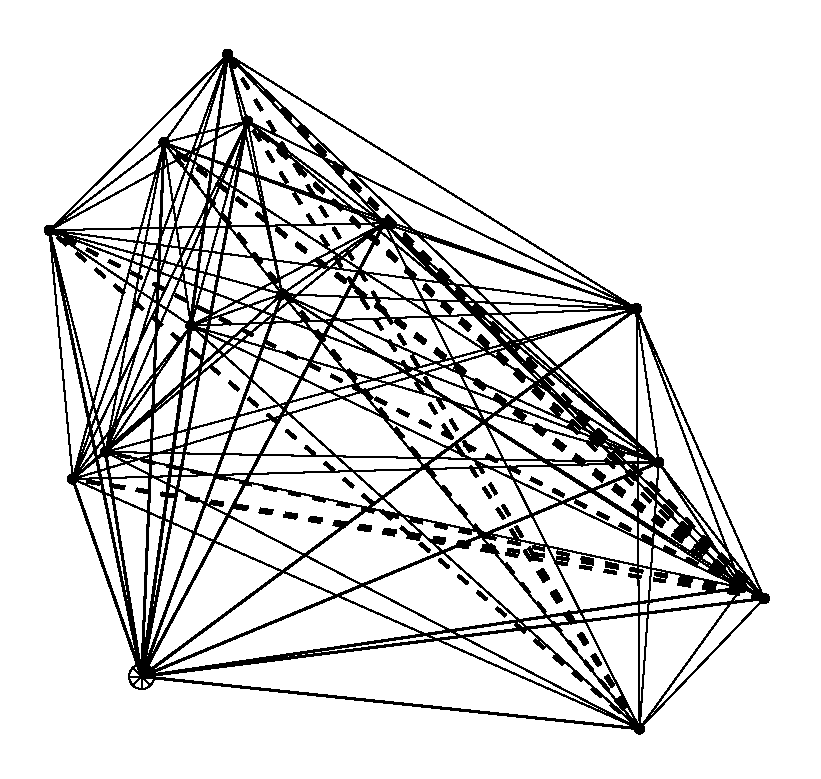
\includegraphics[width=0.4\textwidth]{DistEx.eps}\\
  \caption{the subgraph in one step of GB-NLS. asterisk point: to be determined, dot points: determined, bold and normal solid lines: known distances, broken lines: computed distances}\label{fig:DistEx}
\end{figure}

In GB-NLS, the first step is to compute the unmeasured distances among the fixed points through calculated coordinates (broken lines in Figure \ref{fig:DistEx}), after that, all the distances among these $l+1$ points are known, therefore Matrix Decomposition Method introduced in Subsection \ref{subsec:MatDcomp} can be used to determine point $j$, and adjust these $l$ determined points slightly at the same time. The adjustment usually is tiny but very important, because it provides the chance to mend the inaccurate localizations determined in previous steps when new distance information is involved, while in GB-LLS a point is permanently fixed once it is determined.


\section{our Algorithm}\label{sec:alg}
%\subsection{Motivation}
Compare to SDP relaxation-based algorithms, Geometric Buildup methods (GB-LLS and GB-NLS) are extremely fast since small-sized subproblem is solved at each step. Nevertheless, the original Geometric Buildup algorithms can only tolerate very small noises in distances, usually less than $0.01\%$, even for the state-of-the-art one \cite{Sit2009}, which is not practical in real world applications. In particular, even for the exact distance case, accumulation of round error may destroy the conformation when the number of the atoms is large (more than several thousands), the situation is even worse in the noisy distances case. The initial motivation of this work is to develop some new techniques to overcome this shortage. The proposed algorithms can be viewed as enhanced GB algorithms. Another angle to view our algorithm is that our aim to solve a difficult error function minimization problem, which is a global minimization problem with tremendously many local minimizer, and the layout of GB algorithms serves as a good initial point. All in all, both the Buildup process and the optimization process are equivalently substantial to make the novel algorithm fast and accurate.

In the rest of this section, we first give the analysis of errors in the original GB algorithms, then our strategy to choose the new point and also the optimization subproblems are introduced. Finally a complete description of the novel algorithm is presented.

\subsection{Why does numerical error matter?}
%We are facing large-scale real application problems, computer programs are necessary to finish the complex computations involved. Nevertheless, when the result is obtained through limited-precision float-point computations, we should be very careful because small round errors may ruin a theoretically perfect algorithm. We give the following simple example to illustrate this argument.
%
%Define a one-variable function $f: [0,1]\rightarrow [0,1]$ by
%\begin{equation}
%f(x)=\left\{
%\begin{array}{ll}
%2x,  & 0\leq x \leq 1/2, \\
%2x-1, & 1/2<x\leq 1. \\
%\end{array}
%\right.
%\end{equation}
%the simple iterative scheme is given by $x_{k+1} = f(x_k)$, therefore if we start at $x_0 = 0.4$, the iteration should cycle within 0.4, 0.8, 0.6 and 0.2. However, the real iterative points computed by our 16-digits precision computer is illustrated by Figure \ref{fig:doubling}, the sequence collapses to the original point very quickly (in about fifty iterations). Actually, if you further give an eye on the sequence more carefully, you will find out that the the original round error is very small---in the order of $10^{-15}$, and then quickly accumulated by doubling.
%
%\begin{figure}[htp]
%  \centering
%  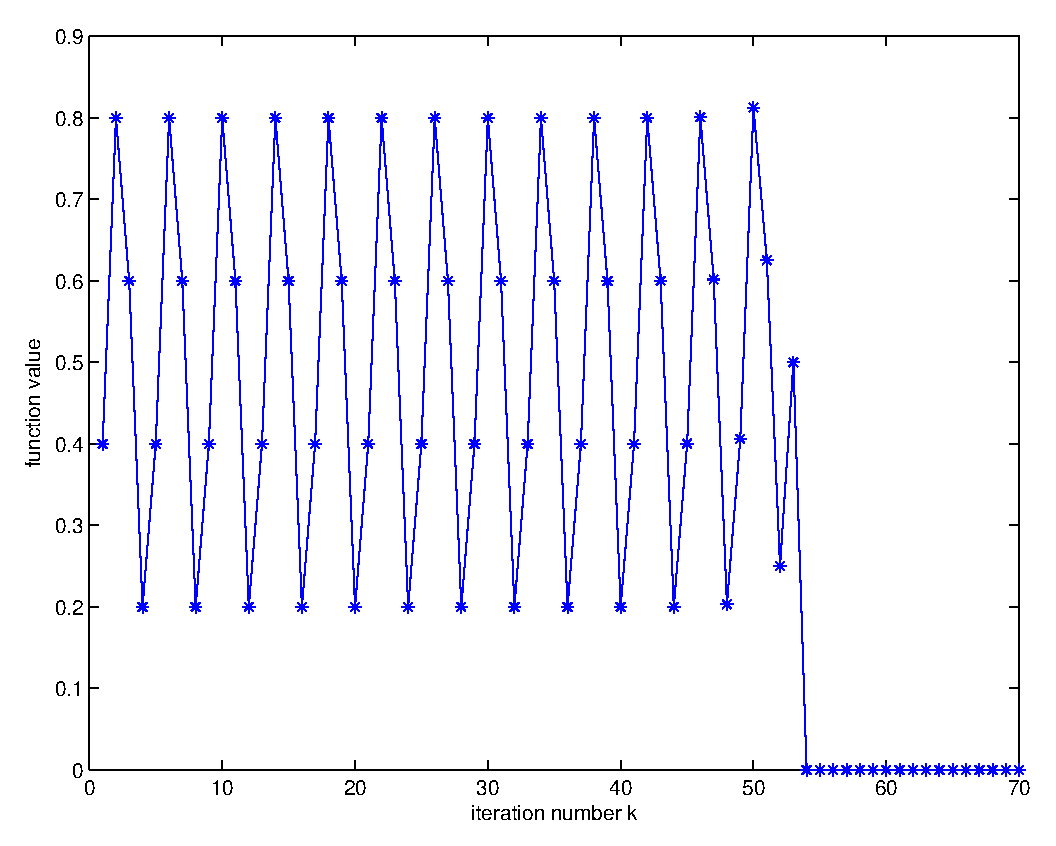
\includegraphics[width=0.4\textwidth]{doubling.eps}\\
%  \caption{A simple example to show how round errors produce large affect on a special iterative algorithm}\label{fig:doubling}
%\end{figure}
%
%In fact, this example give us a clear insight why Geometric Buildup method without linear nor nonlinear least squares does not work for large problems, error accumulation is a key factor in this sequential algorithm. In the noisy distances case, the measured errors are much more larger than the round errors, which makes the problem so challenging.

\begin{figure}[htbp!]
  \centering
  \includegraphics[width=0.4\textwidth]{OriginalOrder.eps}\\
  \caption{RMSD results when GB-LLS is applied to 1MQQ (5681 atoms) with exact distances (cutoff = 6\AA)}\label{fig:OriginalOrder}
\end{figure}

The propagation of numerical errors is a big problem for Geometric Buildup algorithms \cite{Wu2006,Wu2008}, which is also observed in our own numerical experiments. Figure \ref{fig:OriginalOrder} illustrates representative RMSD results (in log10 scale) when GB-LLS is applied to compute 1MQQ (5681 atoms) with exact distances. In theory, this algorithm is guaranteed to produce an accurate conformation \cite{Sit2009}. However, though the RMSD is good at first several hundreds of iterations, it goes up step by step quickly, and becomes totally wrong after about 3500 iterations. Gap exists between theoretical results and computational experiences due to numerical errors, which asks for more robust algorithms to fix it.

\subsection{Analysis of error accumulation in existing Geometric Buildup algorithms}
Here we consider the simple case where the exact distances are given and we use linear least square to determine the new point.

Assume point $j$ is to be determined, which has $l$ distances to the determined points $1,2,\ldots,l$. Let the ground truth be $\widehat{x}_i$, the computed coordinates be $x_i$, and denote location error of point $i$ by $\delta x_i=x_i-\widehat{x}_i$. We further assume $\delta x_i=O(\delta x)$.

Recall that we need solve $\min_{x_j} \|Ax_j-b\|$, where
\be A = 2[(x_{i+1}-x_i)^T], b=[(\|x_{i+1}\|^2-\|x_i\|^2)-(d_{i+1,j}^2-d_{ij}^2)],~i=1,2,\ldots,l-1.\ee
Then we have
\begin{align}
  \|x_{i+1}\|^2-\|x_i\|^2 & = \|\widehat{x}_{i+1}+\delta x_{i+1}\|^2-\|\widehat{x}_i+\delta x_i\|^2    \\
   & = \|\widehat{x}_{i+1}\|^2-\|\widehat{x}_i\|^2 + 2\widehat{x}_{i+1}\delta x_{i+1} - 2\widehat{x}_i\delta x_i + \delta x_{i+1}^2-\delta x_i^2.
\end{align}
Therefore, $A=\widehat{A}+O(\delta x),~~b=\widehat{b}+O(\delta x)$
\begin{align}
  \|Ax_j-b\| & =\|(\widehat{A}+\delta A)(\widehat{x}_j+\delta x_j)-(\widehat{b} + \delta b)\| \\
   & =\|\widehat{A} \delta x_j + O(\delta x)\|.
\end{align}
From the analysis above, we know that the error in each buildup step comes from three aspects: (1) the error inherits from previous calculation, which is hidden in $A$ and $b$ and is the dominant error in most of the buildup steps. (2) the numerical error caused by ill-conditional coefficient matrix $A$, which arises only in a small number of steps but sometimes leads to large error. (3) round error existing in all limited-precision computations.

\subsection{Strategy to choose the newly added point}
Remind that the Geometric Buildup algorithms determine points one by one, which use the coordinates of the determined points and the distances between unknown point to determined points, hence it is obvious that the accuracy of the determined points affect that of subsequent determined points heavily, which makes the computation order very important. In the original GB methods, the default order of the atoms in PDB file (which will be explained in the numerical results part) is used. This kind of structure information is useful but unavailable for real world problems, in which only distances are measured or estimated \cite{Dong2002}. We would like to design a rule that is efficient but solely depend on the given distances, therefore, it is realistic.

Based on the analysis and discussion before, we propose to exploit the following two kinds of information to choose point $j$ to be determined.
\begin{itemize}
    \item (structure information)%: the largest number of known distances \\
    ~~Let $\mathcal{Y}$ be index set of determined points and $\mathcal{N} = \{1,2,\ldots,n\}\backslash \mathcal{Y}$ the undetermined ones, we define
    \be p(i) = \sharp \{d_{ik}\neq 0: k\in \mathcal{Y}\}, ~~for~i\in \mathcal{N}, \label{rule1} \ee
    and further define
    \be \mathcal{I} = \{i: p(i) = \max_{k\in \mathcal{N}} ~p(k)\}, \label{rule2}\ee
    where $p(i)$ is the the number of known distances to the determined points for undetermined point $i$, and $\mathcal{I}$ is the index set of points which have maximal number of known distances.
    \item (distance information)%: closest to the determined points \\
    ~~We choose $j$ satisfying
    \be j = \arg\min_{i\in \mathcal{I}} \sum_{k\in \mathcal{Y}} d_{ik}, \label{rule3}\ee
    which is closest to the determined points in terms of total distances among all the points in $\mathcal{I}$.
\end{itemize}
Intuitively, we choose the point that has the maximal number of distances and is closest to the determined points at the same time. The reason why we need the second rule is that usually there are more than one point satisfying the first rule, randomly choose one point from these points makes the algorithm unstable and unpredictable.

The benefits of this computational order include but are not limited to the following several aspects. (1) The oscillation is removed. In the original GB algorithms, we often observe that the buildup process goes far away and then comes back, this phenomenon disappears under our rules. (2) As a result of (1), we actually have the potential to exploit more number of distances than the original algorithms, which is desired because more distances means we have larger chance to dismiss the measure errors existing in the distance data. (3) The whole algorithm is more stable, here by stable we mean that the condition number of the coefficient matrix in least-quare subproblem is reasonably good, therefore, the numerical difficulty of solving the subproblem is reduced. This is verified by the numerical tests.

\begin{figure}[htp]
  \centering
  \includegraphics[width=0.4\textwidth]{CompOrder.eps}\\
  \caption{A simple example to illustrate the importance of computaional order}\label{fig:CompOrder}
\end{figure}

We construct a simple 2D example in Figure \ref{fig:CompOrder} to illustrate the importance of the computational order. In this example, we have six points, whose serial numbers and locations are shown in the graph, where the line determined by point 1 and 2 is horizontal. What we know are the distances denoted by solid lines. We apply GB-LLS to this instance, points 1,2,3 are determined first as base points, and points 4,5,6 are then determined one by one. It seems perfect but has potential risks. Assume $d_{34}$ is noisy such that point 4 is slightly perturbed under the horizontal line. If we only look at the first four points, the layout is still acceptable because only small error exist in point 4. We then determine point 5 based on the locations of points 1,2,4, it is also under horizontal line, which brings large error to this point. Finally point 6 can not be correctly determined either. The reason why small error perturbation in point 4 leads to large error in point 5 is that points 1,2,4 are almost in the same line, therefore the coefficient matrix $A$ for determining point 5 is ill-conditioned.

Now we show how these risks disappear under our rules. The first two steps are the same, the difference is that point 6 is determined before point 5, since they both have three distances to the determined points---1,2,3,4, but point 6 is closer to them. After point 6 is determined, point 5 can also be determined stably because now four distances are used and points 1,2,4,6 make up a table base. This man-made instance shows the advantage of our strategies, which is also verified by the tests on real protein data.

\subsection{Error function minimization procedures}
\subsubsection{Subproblems}
We first introduce the concept of induced subgraph. Let $G=(V,E)$ be a graph, $V'\subseteq V$ be a subset of the vertex set, then $G(V')=(V',E')$ is the induced subgraph of $G$, where $E'=\{(i,j)\in E: i\in V', j\in V'\}$.

After each buildup step, we propose to add an optimization step on the subgraph $G(j\cup N(j))$, where $N(j)=\{k: d_{jk}\neq 0\}$ is the neighbourhood of point $j$, i.e., we further solve the following subproblem
\be \min  f(x_{j\cup N(j)}), \label{prob:sub}\ee
where $f(\cdot)$ is a certain error function defined on the induced subgraph $G(j\cup N(j))$, the deviations are added on the edges in $E'$. We choose $f(\cdot)$ as $Stress(\cdot)$ in \reff{eqn:stress} with $\omega_{ij}=1$ in this paper.

%\subsubsection{Comments and further discussion on error function}
Notice that the objective function in \reff{prob:sub} has the same form with the final problem but only consists of the given distances among point $j$ and its neighbours. Since the problem is usually small-sized (no more than  several tens in protein structure determination) and the buildup step produces a high-quality initial point, the subproblem \reff{prob:sub} is usually solved within a small number of iterations to high accuracy, therefore, the computational cost brought by this optimization step is not too much.

From another point of view, the subproblem can be viewed as a tradeoff between linear and nonlinear least square in terms of the usage of distances information. As we have mentioned before, GB-LLS utilizes only $l$ distances (too few) and GB-NLS utilizes not only given distances but also computed ones (too many), and we use a balanced approach between these two extreme methods. The benefits are obvious. We keep the advantage of GB-NLS---stability and the chance to adjust the determined points according to the freshly determined point and distances involved, and avoid the risks of accumulating old errors when use computed distances. Moreover, while matrix decomposition method works on the transformation of distance equations, our method works on squared deviations of the distances directly.

\subsubsection{Solution algorithm}
The derivative of of $Stress$ can be computed directed as following,
\be \frac{\partial Stress}{\partial x_i}=2\sum_{j\in N(i)} \Big(1-\frac{d_{ij}}{\|x_i-x_j\|}\Big)(x_i-x_j), \label{gradient}\ee
where $N(i)$ is the neighbourhood of point $i$ as defined before.

In this paper, we basically exploit gradient method with Barzilai-Borwein (BB) stepsize \cite{BB1988} to solve \reff{gradient}. We also incorporate with a Armijo backtracking line search \cite{Armijo1966,Sun2006} if BB step makes no improvement in a succession of $M$ steps to ensure the convergence.

\textbf{Armijo Line search} Let $\alpha = \delta\beta^i$, where $\delta>0$ is the initial stepsize, $i$ is the minimal nonnegative integer such that
\be f(x)-f(x+\delta\beta^id)\geq -b\delta\beta^i d^T\nabla f(x), \ee
where $b\in (0,1)$ is a parameter, and $d$ is the search direction.

During the iterations, $\delta^k=\frac{\|s^{k-1}\|^2}{{s^{k-1}}^Ty^{k-1}}$ is the long BB stepsize in $k$-th iteration, where $s^k=x^k-x^{k-1}$, $y^{k-1}=g^k-g^{k-1}$, $x^k$ is the iteration point and $g^k$ is the gradient. The iteration scheme is given by
\be x^{k+1} = x^k + \alpha^kd^k.\ee

%We also apply the following nonmonotone line search technique to make our algorithm have to ability to escape from some not so good local minimizers.

\subsection{Framework of our algorithms}
Now we summarize the discussions before and give a complete description of our proposed algorithms.
%
%\begin{algorithm}[H]
%\SetKwInOut{Input}{input}\SetKwInOut{Output}{output}
%\Input{A symmetric distance matrix $D$} %to specify part of the pairwise distances}
%\Output{index set of determined points and coordinate matrix $X$}
%%\vskip1mm
%Find a maximal clique that are not in the same plane\;
%Use Matrix Decomposition Method to determine these points\;
%%Repeat:
%
%\While{not all the points are determined}{
%Find point $j$ according to \reff{rule1}, \reff{rule2} and \reff{rule3}\;
%\eIf{$l=p(j)\geq 4 ~\&~ N(j) \textrm{ not in the same plane}$}
%{Determine $x_j$ by linear \reff{LLS} or nonlinear least square \reff{NLS}\;
%Adjust the locations of points $j\cup N(j)$ by solving \reff{prob:sub}.
%}
%{No more point can be uniquely determined\;
%Return the determined index set and coordinates, stop.}
%}
%\caption{Enhanced Geometric Buildup for sparse noisy anchor-free Distance Geometry Problem}
%\end{algorithm}

\begin{algorithm}[H]
\begin{enumerate}[Step 1]
  \item Find a maximal clique that are not in the same plane, and use Matrix Decomposition Method (Subsection \ref{subsec:MatDcomp}) to determine them. Set $\mathcal{T}=$ \{index of points in the clique\}.
  \item Find index $j$ according to \reff{rule1}, \reff{rule2} and \reff{rule3}. If $l=p(j)\geq 4$ and the points in $N(j)$ are not in the same plane, go to Step 3, go to Step 5 otherwise.
  \item Determine $x_j$ by linear least quare (Subsection \ref{LLS}) or nonlinear least square (Subsection \ref{NLS}), then solve \reff{prob:sub} to adjust $x_{j\cup N(j)}$. \\Set $\mathcal{T}=\mathcal{T}\cup \{j\}$.
  \item If all the points are determined, go to Step 5, go to Step 2 otherwise.
  \item Solve \reff{prob:error} with variables in $\mathcal{T}$, stop.
\end{enumerate}
\caption{Geometric Buildup-based Error Minimization (GBEM) algorithms for sparse noisy anchor-free Distance Geometry Problem}
\label{alg:EGB}
\end{algorithm}
According to different least square techniques we exploit in Step 3, we refer our proposed algorithms as GBEM-LLS and GBEM-NLS, respectively.

%
%\subsection{Subspace point of view}
%Subspace is not a new concept but somehow a new aspect to view an algorithm \cite{Yuan2007}, and also useful philosophy to design algorithm to solve large-scale problems. We now focus the optimization problems solved in Algorithm \ref{alg:EGB} and explain this algorithm in subspace fashion.
%
%Our final task is to solve \reff{prob:error} (Step 5), which is an optimization problem with $n$ points thus totally $n\times  d$ variables. Instead of solving this difficult problem directly, we actually choose to iteratively minimize this function restricted at subspace $x_{j\cup N(j)}$ (Step 3), which is much easier to solve.
%
%\subsection{Convergence}
%The convergence of Algorithm \ref{alg:EGB} to a local minimizer is guaranteed by the standard theory of gradient method with Barzilai-Borwein step size \cite{BB1988,Sun2006}. However, as we have stated before, this local convergence is of little meaning in practice. On the other hand, the convergence to global solution is not easy to prove (actually, we believe there exist counterexamples, but this kind of example is meaningless for real applications, we do not waste our time to do that). Numerical results in next section will show that our algorithm can converge to global solution or very close to optimal solution in many instances.

\section{Numerical experiments}\label{sec:num}
We have not found any open data sets about distance geometry problem. Even for the protein structure determination problem, different simulated data are used in different papers. For example, a part of the upper and lower bounds of distances under 6\AA ~(1\AA ~= $10^{-10}$m)~ are used in DAFGL \cite{Biswas2008}. In the enhanced DISCO \cite{Fang2013}, 20\% of pairwise noisy distances less than 6\AA ~are tested, but they have incorporated distance information derived from chemistry knowledge. So it is not easy to compare our algorithms to many others because the problem settings are different and the simulated errors are added randomly. We only compare our algorithms with the original state-of-the-art Geometric Buildup algorithms in \cite{Sit2009}, especially show the ability to handle large noisy distances.

In this section, we will first introduce how we construct test problems to simulate real distance data in proteins, and then give the detailed numerical results. In addition, some conclusions and discussions are presented based on the experiment results.

\subsection{Problem setting}
We first download the protein data from Protein Data Bank (PDB) \cite{Berman2000} (http://www.pdb.org), which is an archive of experimentally determined three-dimensional protein structures and contains 3D biological macromolecular structure data of proteins. According to the coordinates in the PDB files, we use $disk~ graph~ model$ to construct the distance matrices, which is to say, we assume $d_{ij}$ is known if it is less than or equal to the prescribed cutoff (usually 5\AA ~or 6\AA, where 6\AA ~is roughly the maximum distance that NMR techniques can measure between two atoms \cite{Biswas2008}). In this way we simulate the real situation that only distances under a certain cutoff can be measured due to the limitation of biological techniques.

In real applications, the measured distances tend to be contaminated by noises, we simulate this by adding normally or uniformly distributed multiplicative perturbations to the exact distances as following,
$$d_{ij} = \bar{d}_{ij}(1+\delta_{ij}*nl)$$
where $\bar{d}_{ij}=\|\bar{x}_i-\bar{x}_j\|$ is the exact distance between point $i$ and point $j$, $\delta_{ij}$ is a random number obeying a certain given distribution. For example, $\delta_{ij} \sim N(0,1)$ if the standard normal distribution is used \cite{Biswas2008}, and $\delta_{ij} \sim U[-1,1]$ if the uniform distribution is used \cite{Sit2009}. We present results to deal with normally distributed noises in the paper, and omit the similar results for the latter case. $nl$ is the noise level we set, which are $1\%, 5\%$, or $10\%$ to represent low, median and high noise level, respectively.

\subsection{Results and discussions}
We apply GBEM-LLS and GBEM-NLS to the distance matrices. Notice that the only information we need in our algorithms is distances, and the correct coordinates of the points are only used to examine the accuracy of the results, which are measured by the Rooted Mean Squared Deviation (RMSD) value as following,
\be RMSD(X,Y) = \min_{Q,T}\{ \|Y-XQ-T\|_{F}/\sqrt{n}: \Tran{Q}Q=I\}, \ee
where $X\in \Real^{n\times 3}$, $Y\in \Real^{n\times 3}$ are the computed coordinate matrix and true one, respectively, $T$ is a translation vector and $Q$ is an orthogonal matrix as the constraint states. Basically, we try to move $X$ through rigid transformations (translations, rotations and possible reflections) to coincide with $Y$ as much as possible, and RMSD measures the minimal deviations. Notice that the RMSD criterion can only be used to examine the performance of the algorithm and is impractical in real applications because the ground truth coordinates $Y$ is needed, which is unattainable for an unsolved problem. Instead, error function related criteria (such as function value or norm of the gradient) are used as stopping rules in various algorithms. One such kind of criterion is given in \cite{Biswas2008} as following,
\be LDME = \Big(\frac{1}{|E|} \sum_{(i,j)\in E}\big(\|x_i-x_j\|-d_{ij}\big)^2\Big)^{1/2}\ee
But just as the authors point out in paper \cite{Biswas2008}, LDME (local
distance matrix error) is more practical but less reliable in evaluating the true accuracy of the constructed configuration, which means smaller LDME does not necessarily mean more accurate localization, so we do not report function values in the main results tables, though we use it as a stopping criterion in the optimization step.

Our programs are written in Matlab, no MEX files are involved, though the most costly part is the gradient computation with loops, which can be speeded up by writing in C and compiling through MEX files. The programs are run in Matlab R2013b version 8.2 on a Dell PC, with 2.83 GHz CPU and 4.00 GB RAM.

%\newcolumntype{R}{>{\flushright\arraybackslash}X}
%\renewcommand\arraystretch{0.85}
\setlength{\tabcolsep}{9.5pt}
\begin{table}[htb!]
\centering
\footnotesize{
\caption{Problems information summary}
\begin{tabular}{lrrrrrrrrr}
  \toprule
   &  &  \multicolumn{4}{c}{cutoff = 5\AA} & \multicolumn{4}{c}{cutoff = 6\AA} \\
  \cmidrule(r){3-6}\cmidrule(r){7-10}
  \hd{ID}& \hd{Num} &  & \multicolumn{3}{c}{degree} &  & \multicolumn{3}{c}{degree}\\
  \cmidrule(r){4-6} \cmidrule(r){8-10}
  & & \hd{per} & max & min & avr &\hd{per} & max & min & avr \\
  \midrule
  1PTQ &  402 & 5.46 & 38 & 4 & 21.9 & 8.79 & 61 &  6& 35.3  \\
  1HOE &  558 & 4.05 & 38 & 6 & 22.6 & 6.55 & 65 & 11& 36.5  \\
  1LFB &  641 & 3.40 & 40 & 5 & 21.8 & 5.57 & 59 &  8& 35.7  \\
  1PHT &  811 & 3.35 & 48 & 5 & 27.1 & 5.37 & 75 &  7& 43.5  \\
  1POA &  914 & 2.51 & 39 & 4 & 22.9 & 4.07 & 67 &  8& 37.2  \\
  1AX8 & 1003 & 2.30 & 39 & 5 & 23.0 & 3.74 & 59 &  7& 37.5  \\
  4MBA & 1083 & 2.17 & 39 & 5 & 23.5 & 3.56 & 60 &  5& 38.5  \\
  1F39 & 1534 & 1.47 & 40 & 5 & 22.6 & 2.43 & 62 &  7& 37.2  \\
  1RGS & 2015 & 1.12 & 41 & 3 & 22.6 & 1.87 & 66 &  4& 37.7  \\
  1KDH & 2846 & 0.83 & 43 & 4 & 23.6 & 1.36 & 64 &  5& 38.8  \\
  1BPM & 3671 & 0.66 & 42 & 3 & 24.4 & 1.12 & 64 &  4& 40.9  \\
  1RHJ & 3740 & 0.65 & 40 & 4 & 24.4 & 1.10 & 61 &  5& 41.2  \\
  1HQQ & 3944 & 0.60 & 40 & 3 & 23.7 & 1.00 & 64 &  5& 39.5  \\
  1TOA & 4292 & 0.56 & 39 & 3 & 24.0 & 0.94 & 62 &  4& 40.1  \\
  1MQQ & 5681 & 0.44 & 44 & 5 & 25.2 & 0.75 & 66 &  7& 42.4  \\
  1HMV & 7398 & 0.32 & 42 & 3 & 23.3 & 0.52 & 67 &  4& 38.7  \\
  1I7W & 8629 & 0.29 & 48 & 3 & 24.7 & 0.47 & 73 &  5& 40.9  \\
  \toprule
\end{tabular}\\[-3mm]
\label{table:probinfo}
\begin{flushleft}
ID---protein ID in PDB, Num---number of atoms in each protein, per---percentage of the known distances among all the pairwise distances, degree---maximum/minimum/average degree of all the points
\end{flushleft}
}
\end{table}
We have tested GBEM-LLS and GBEM-NLS on all the 17 proteins mentioned in \cite{Biswas2008} and \cite{Sit2009}, where the number of atoms ranging from 402 to 8629. We summarize the problems information in Table \ref{table:probinfo}. The first column in the table is PDB ID, which is the unique identity of a certain protein in PDB. The second column is the number of atoms in each protein. In the third column, we list the sparsity of distance matrix as \cite{Biswas2008}, which is the percentage of the known distances among all the pairwise distances. However, we do not think this is an appropriate criterion to describe the difficulty of the problem. For example, if we make nine copies of a graph (and add a few necessary edges to make it a connected graph), the available distances will be about ten times more (in linear scale), but the total pairwise distance is in order $n^2$, i.e., about 100 times more, hence the sparsity of the distance is significantly increased, while the real difficulty to solve the problem remains almost the same, except for the time the algorithms take. This example shows that it contradicts with the intuition that the sparser the distance, the much more difficult the problem. Actually, we think sparsity is a meaningful criterion only when the number of the points in different graphs are the same or in the same order. Therefore, we also list the maximal, minimal and average degree of the graphs in the subsequent three columns. Degree information can properly reveal the difficulty of the problem, especially for our algorithms. The smaller the degrees, the few information we can exploit for each individual point, thus the more difficult the problem. The last four columns are similar, where we increase the cutoff from 5\AA ~to 6\AA, hence more distances are known.

\setlength{\tabcolsep}{5.5pt}
\begin{table}[htb!]
\centering
\scriptsize{
\caption{RMSD values (in \AA) of simulated proteins with exact distances}
\begin{tabular}{lrcccccccc}
  \toprule
   &  & \multicolumn{4}{c}{cutoff = 5\AA}
   & \multicolumn{4}{c}{cutoff = 6\AA} \\
  \cmidrule(r){3-6} \cmidrule(r){7-10}
  \hd{ID} & \hd{Num} & \multicolumn{2}{c}{LLS} & \multicolumn{2}{c}{NLS} & \multicolumn{2}{c}{LLS} & \multicolumn{2}{c}{NLS} \\
  \cmidrule(r){3-4} \cmidrule(r){5-6} \cmidrule(r){7-8} \cmidrule(r){9-10}
   & & \hd{GB} & \hd{GBnew} & \hd{GB} & \hd{GBnew} & \hd{GB} & \hd{GBnew} & \hd{GB} & \hd{GBnew} \\
  \midrule
  1PTQ &  402 & 1.4e$+$00 & 6.5e$-$13 & 5.5e$-$14 & 5.1e$-$14 & 2.6e$-$09 & 2.8e$-$14 & 5.0e$-$14& 2.9e$-$14  \\
  1HOE &  558 & 5.8e$-$02 & 3.0e$-$13 & 1.6e$-$13 & 2.4e$-$14 & 3.1e$-$09 & 3.8e$-$14 & 2.7e$-$13& 2.0e$-$14  \\
  1LFB &  641 & 2.0e$-$02 & 9.3e$-$14 & 9.5e$-$14 & 3.1e$-$14 & 2.1e$-$10 & 4.6e$-$14 & 5.5e$-$14& 2.1e$-$14  \\
  1PHT &  811 & 1.2e$+$01 & 2.0e$-$12 & 1.1e$-$13 & 6.3e$-$14 & 8.2e$-$09 & 9.3e$-$14 & 1.8e$-$13& 5.7e$-$14  \\
  1POA &  914 & 6.6e$+$00 & 8.2e$-$13 & 3.2e$-$13 & 7.4e$-$14 & 1.9e$-$09 & 2.8e$-$13 & 1.5e$-$13& 4.7e$-$14  \\
  1AX8 & 1003 & 5.2e$+$00 & 1.1e$-$11 & 4.0e$-$13 & 3.3e$-$14 & 1.8e$-$05 & 5.4e$-$14 & 4.6e$-$12& 3.0e$-$14  \\
  4MBA & 1083 & 4.9e$+$00 & 3.6e$-$12 & 1.8e$-$13 & 8.2e$-$14 & 3.8e$-$06 & 1.2e$-$13 & 2.6e$-$13& 6.9e$-$14  \\
  1F39 & 1534 & 1.4e$+$00 & 6.7e$-$13 & 7.9e$-$13 & 5.2e$-$14 & 6.3e$-$08 & 2.1e$-$13 & 1.9e$-$13& 4.7e$-$14  \\
  1RGS & 2015 & 2.0e$+$01 & 2.5e$-$10 & 8.3e$-$12 & 2.2e$-$13 & 1.1e$-$01 & 2.1e$-$12 & 2.4e$-$12& 1.7e$-$13  \\
  1KDH & 2846 &     -     & 7.2e$-$11 &     -     & 1.9e$-$13 &     -     & 5.6e$-$13 &     -    & 1.5e$-$13  \\
  1BPM & 3671 & 6.4e$+$04 & 9.6e$-$10 & 8.1e$-$11 & 1.3e$-$13 & 3.6e$-$02 & 3.3e$-$13 & 1.0e$-$11& 1.0e$-$13  \\
  1RHJ & 3740 &     -     & 3.7e$-$09 &     -     & 6.4e$-$14 &     -     & 3.9e$-$13 &     -    & 8.2e$-$14  \\
  1HQQ & 3944 &     -     & 1.3e$-$09 &     -     & 5.3e$-$14 &     -     & 9.0e$-$13 &     -    & 6.8e$-$14  \\
  1TOA & 4292 &     -     & 3.4e$-$09 &     -     & 9.5e$-$14 &     -     & 4.9e$-$12 &     -    & 2.2e$-$13  \\
  1MQQ & 5681 &     -     & 6.8e$-$11 &     -     & 1.6e$-$13 &     -     & 6.1e$-$13 &     -    & 6.8e$-$14  \\
  1HMV & 7398 & 1.2e$+$03 & 6.1e$-$07 & 1.1e$-$08 & 3.8e$-$13 & 3.5e$+$01 & 5.6e$-$11 & 5.5e$-$07& 6.0e$-$13  \\
  1I7W & 8629 &     -     & 2.0e$-$06 &     -     & 3.8e$-$13 &     -     & 6.4e$-$12 &     -    & 2.7e$-$13  \\ \toprule
\end{tabular}\\[-4mm]
\label{table:exact}
\bl ID---protein ID in PDB, Num---number of atoms in each protein, LLS---Linear Least Square, NLS---Nonlinear Least Square, GB---the original Geometric Buildup algorithms, GBnew---Geometric Buildup algorithms with the proposed computation order \el
}
\end{table}

We first compare Geometric Buildup algorithms equipped with the proposed computation order (we refer it as GBnew) with the original Geometric Buildup algorithms to show the efficiency of our strategies to define the computation order. Notice that the optimization steps are omitted in these tests. The RMSD results are reported in Table \ref{table:exact}, where results of the original GB algorithms are copied from Table 2 and Table 3 in \cite{Sit2009}, and '-' means that the proteins are not tested by them. From the table, we can see that GBnew achieves better results than the original algorithms, especially when the data are very sparse (cutoff=5\AA), the original algorithms can not generate meaningful layout for many proteins but our algorithms can. We have also tested proteins with cutoff 7\AA ~and 8\AA~ as \cite{Sit2009}, all the instances are determined accurately, even for those they can not determine. Since these settings are not practical in real problems, we do not report the details. Moreover, the increased CPU time are negligible compared to the original algorithms. For instance, a 8629 atoms protein---1I7W with cutoff 6\AA ~is determined by GBnew-LLS in 19.0 seconds.

Before presenting the numerical results on large noisy distances, we have to point out that the results are related to the parameter settings in the algorithms. For example, different maximum iteration number or different small tolerance (for example $10^{-2}$ or $10^{-3}$) the gradient achieves usually give different RMSD and CPU time results. In most of the cases, smaller tolerance or larger maximum iteration number gives more accurate (i.e., smaller RMSD) results, but takes longer time. One counterexample we encounter is when we compute 1MQQ with cutoff 5\AA~ and noise level 5\%, we increase the tolerance from $10^{-2}$ to $10^{-3}$, then we obtain much smaller function value, but larger RMSD, and of course the time it takes is longer. Usually we can always adjust the parameters to get better results for one particular protein, but we do not do that because for real problems, what we can do is setting the parameters and obtain results, not the opposite. Throughout the paper, the results are generated by uniform parameter settings in all the noisy cases.

\setlength{\tabcolsep}{4pt}
\begin{table}[htb!]
\centering
\footnotesize{
\caption{RMSD (in \AA) and CPU time (in seconds) of simulated proteins with cutoff = 5\AA, noise level = 1\% and 5\%}
\begin{tabular}{lrrrrrrrrrr}
  \toprule
   & & & \multicolumn{4}{c}{noise level = 1\%}
   & \multicolumn{4}{c}{noise level = 5\%} \\
  \cmidrule(r){4-7} \cmidrule(r){8-11}
  \hd{ID} & \hd{Num} & \hd{nDet}& \multicolumn{2}{c}{LLS} & \multicolumn{2}{c}{NLS} & \multicolumn{2}{c}{LLS} & \multicolumn{2}{c}{NLS} \\
  \cmidrule(r){4-5} \cmidrule(r){6-7} \cmidrule(r){8-9} \cmidrule(r){10-11}
   & & & \hd{RMSD} & \hd{CPU} & \hd{RMSD}  & \hd{CPU} & \hd{RMSD}  & \hd{CPU} & \hd{RMSD}  & \hd{CPU} \\
  \midrule
  1PTQ &  402 &  402 & 1.1e$-$01 &  1.0 & 6.0e$-$02 &  1.1 & 2.0e$-$01 &   2.1 & 2.1e$-$01&   2.2  \\
  1HOE &  558 &  558 & 1.6e$-$01 &  1.7 & 3.7e$-$02 &  1.6 & 1.9e$-$01 &   3.6 & 2.6e$+$00&   4.1  \\
  1LFB &  641 &  641 & 1.6e$-$01 &  1.9 & 9.6e$-$02 &  1.9 & 5.9e$-$01 &   3.1 & 3.6e$+$00&   4.7  \\
  1PHT &  811 &  806 & 2.2e$-$01 &  2.6 & 6.1e$-$02 &  3.0 & 3.2e$-$01 &   6.0 & 1.9e$-$01&   5.8  \\
  1POA &  914 &  914 & 2.0e$-$01 &  2.9 & 8.8e$-$02 &  2.7 & 2.5e$-$01 &   6.4 & 4.1e$-$01&   5.9  \\
  1AX8 & 1003 & 1003 & 2.3e$-$01 &  3.8 & 7.9e$-$02 &  3.3 & 4.3e$-$01 &   8.8 & 8.0e$+$00&  10.8  \\
  4MBA & 1083 & 1080 & 2.1e$-$01 &  3.6 & 1.5e$-$01 &  4.3 & 2.6e$-$01 &   9.2 & 2.4e$+$00&  10.7  \\
  1F39 & 1534 & 1534 & 3.4e$-$01 &  5.2 & 1.3e$-$01 &  5.0 & 6.3e$-$01 &  12.7 & 5.1e$-$01&   9.5  \\
  1RGS & 2015 & 2010 & 9.5e$-$01 & 10.2 & 1.8e$-$01 &  7.2 & 2.9e$+$00 &  17.7 & 7.9e$+$00&  20.9  \\
  1KDH & 2846 & 2846 & 3.4e$-$01 & 17.7 & 2.3e$-$01 & 17.0 & 2.6e$+$00 &  28.5 & 1.4e$+$01&  34.6  \\
  1BPM & 3671 & 3668 & 4.5e$-$01 & 23.3 & 9.5e$-$02 & 16.4 & 7.4e$-$01 &  35.4 & 2.6e$-$01&  32.7  \\
  1RHJ & 3740 & 3740 & 1.3e$-$01 & 18.2 & 9.4e$-$02 & 18.5 & 4.4e$-$01 &  36.8 & 1.4e$+$01&  50.5  \\
  1HQQ & 3944 & 3938 & 1.7e$-$01 & 19.0 & 1.0e$-$01 & 17.5 & 4.3e$-$01 &  37.2 & 4.5e$-$01&  34.6  \\
  1TOA & 4292 & 4280 & 4.0e$-$01 & 29.4 & 1.2e$-$01 & 22.4 & 1.0e$+$00 &  43.6 & 5.1e$-$01&  34.4  \\
  1MQQ & 5681 & 5681 & 3.3e$-$01 & 47.8 & 1.0e$-$01 & 35.0 & 5.1e$+$00 &  70.2 & 3.6e$+$00&  73.0  \\
  1HMV & 7398 & 7389 & 2.6e$+$00 & 70.7 & 3.8e$-$01 & 54.3 & 3.7e$+$00 &  83.0 & 9.7e$+$00& 100.3  \\
  1I7W & 8629 & 8624 & 1.9e$+$00 & 79.0 & 1.0e$+$00 & 69.8 & 2.3e$+$01 & 109.4 & 6.2e$+$00& 121.1  \\ \toprule
\end{tabular}\\[-4mm]
\label{table:cut5}
\bl ID---protein ID in PDB, Num---number of atoms in each protein, nDet---number of determined atoms by our algorithms, LLS---GBEM with Linear Least Square, NLS---GBEM with Nonlinear Least Square, RMSD---RMSD values of computed structures against original ones, CPU---toal CPU time the algorithms cost \el
}
\end{table}

We report our first main numerical results on noisy distances in Table \ref{table:cut5}, where we set cutoff to be 5\AA, and noise level to be 1\% and 5\%. Notice that nDet (number of determined atoms) column is a little smaller than Num column for some proteins, which means our algorithm can not determine all the atoms for these proteins, but only leave out very few, because the distance matrix is so sparse such that these atoms have at most three distances to the determined atoms, thus produces at least two options for the locations and can not be determined uniquely. The RMSD and CPU time results are reported only for the determined points.

Recall that the cutoff equals to 5\AA, the layout is very accurate when RMSD (roughly the average deviation of all the atoms) is in order of $10^{-1}$ or even smaller, is not so good when it is larger than about 2\AA, and is totally wrong when it is in order of $10^{1}$ or larger. From the table, we find that GBEM-NLS generates more accurate configurations than GBEM-LLS when noise level is low---1\%, which is the opposite when noise level is increased to 5\%, where NLS inherits too much errors from previous steps when computing distances to make the subgraph complete. In a word, our algorithms can determine most of the proteins accurately but they also give wrong results in very few cases because the distances are too sparse and the noises are too large.

In term of CPU time the algorithms cost, both algorithms only take a couple of seconds to determine several thousands of points. Even for the two largest proteins with 7398 and 8629 atoms, they only take about one hundred seconds, which is much faster than SDP based algorithms \cite{Biswas2008}. Another observation is that GBEM-NLS takes shorter time to stop than GBEM-LLS if both algorithms have good results.


%The 7th column is the function value of the final computed coordinates, and the 8th column is a very special one, which is the function value that we put the truth coordinates into the error function. If the former value is close to or even less than the later one, which indicates that there is little improvement we can get based on the current error function. The last two columns are the $RMSD$ error and CPU time the whole algorithm takes.

\setlength{\tabcolsep}{2pt}
\begin{table}[htb!]
\centering
\scriptsize{
\caption{RMSD (in \AA) and CPU time (in seconds) of simulated proteins with
cutoff = 6\AA, noise level = 1\%, 5\% and 10\% (All the points are determined)}
\begin{tabular}{lrrrrrrrrrrrrr}
  \toprule
   & & \multicolumn{4}{c}{noise level = 1\%}
   & \multicolumn{4}{c}{noise level = 5\%} & \multicolumn{4}{c}{noise level = 10\%} \\
  \cmidrule(r){3-6} \cmidrule(r){7-10} \cmidrule(r){11-14}
  \hd{ID} & \hd{Num} & \multicolumn{2}{c}{LLS} & \multicolumn{2}{c}{NLS} &
  \multicolumn{2}{c}{LLS} & \multicolumn{2}{c}{NLS}  & \multicolumn{2}{c}{LLS} & \multicolumn{2}{c}{NLS} \\
  \cmidrule(r){3-4} \cmidrule(r){5-6} \cmidrule(r){7-8} \cmidrule(r){9-10}
  \cmidrule(r){11-12} \cmidrule(r){13-14}
   & & \hd{RMSD} & \hd{CPU} & \hd{RMSD}  & \hd{CPU} & \hd{RMSD}  & \hd{CPU}
   & \hd{RMSD}  & \hd{CPU} & \hd{RMSD}  & \hd{CPU} & \hd{RMSD}  & \hd{CPU}\\
  \midrule
  1PTQ &  402 & 4.1e$-$02 &  1.3 & 3.4e$-$02 &   2.2 & 1.6e$-$01 &   2.8 & 1.9e$-$01&   4.3 & 3.1e$-$01 &   4.2 & 3.2e$-$01&   5.8  \\
  1HOE &  558 & 2.8e$-$02 &  1.9 & 2.3e$-$02 &   3.1 & 1.1e$-$01 &   4.2 & 1.0e$-$01&   6.3 & 2.1e$-$01 &   5.9 & 2.0e$-$01&   9.1  \\
  1LFB &  641 & 4.2e$-$02 &  2.2 & 3.8e$-$02 &   3.5 & 1.6e$-$01 &   4.8 & 1.7e$-$01&   8.6 & 3.3e$-$01 &   7.3 & 3.6e$-$01&   8.7  \\
  1PHT &  811 & 1.3e$-$01 &  3.4 & 4.8e$-$02 &   6.7 & 2.2e$-$01 &   7.3 & 1.6e$-$01&  14.7 & 4.8e$-$01 &  10.4 & 4.7e$-$01&  14.4  \\
  1POA &  914 & 4.2e$-$02 &  3.3 & 3.7e$-$02 &   5.8 & 1.7e$-$01 &   7.4 & 4.6e$-$01&  14.1 & 5.0e$-$01 &  10.0 & 5.3e$-$01&  13.9  \\
  1AX8 & 1003 & 5.8e$-$02 &  4.0 & 3.7e$-$02 &   6.2 & 1.3e$-$01 &   8.4 & 1.2e$-$01&  11.9 & 2.3e$-$01 &  11.9 & 2.9e$-$01&  16.2  \\
  4MBA & 1083 & 6.4e$-$02 &  4.8 & 2.9e$-$02 &   7.0 & 1.7e$-$01 &   9.2 & 1.2e$-$01&  13.0 & 2.6e$-$01 &  13.4 & 2.4e$-$01&  19.1  \\
  1F39 & 1534 & 4.6e$-$02 &  6.2 & 3.9e$-$02 &   9.7 & 2.5e$-$01 &  14.0 & 1.8e$-$01&  19.3 & 6.1e$-$01 &  18.1 & 3.5e$-$01&  24.0  \\
  1RGS & 2015 & 1.2e$-$01 &  8.6 & 5.1e$-$02 &  13.6 & 2.9e$-$01 &  18.4 & 2.8e$-$01&  27.2 & 6.0e$-$01 &  29.1 & 4.5e$-$01&  37.3  \\
  1KDH & 2846 & 1.0e$-$01 & 15.2 & 5.3e$-$02 &  22.7 & 1.6e$-$01 &  29.0 & 1.9e$-$01&  40.9 & 3.9e$-$01 &  43.0 & 1.2e$+$00&  51.2  \\
  1BPM & 3671 & 9.4e$-$02 & 20.5 & 3.7e$-$02 &  34.0 & 1.5e$-$01 &  41.4 & 1.4e$-$01&  67.8 & 2.4e$-$01 &  56.0 & 2.8e$-$01&  73.0  \\
  1RHJ & 3740 & 8.1e$-$02 & 22.0 & 2.8e$-$02 &  35.0 & 1.3e$-$01 &  39.9 & 1.2e$-$01&  59.0 & 2.5e$-$01 &  58.3 & 2.8e$-$01&  72.2  \\
  1HQQ & 3944 & 5.8e$-$02 & 20.5 & 3.7e$-$02 &  36.2 & 1.8e$-$01 &  43.0 & 1.9e$-$01&  63.4 & 3.4e$-$01 &  60.3 & 3.6e$-$01&  82.7  \\
  1TOA & 4292 & 8.4e$-$02 & 24.6 & 4.6e$-$02 &  45.3 & 1.8e$-$01 &  48.2 & 1.5e$-$01&  72.3 & 5.6e$-$01 &  72.8 & 4.2e$-$01&  89.2  \\
  1MQQ & 5681 & 4.0e$-$02 & 35.5 & 3.2e$-$02 &  64.8 & 1.1e$-$01 &  67.7 & 1.2e$-$01& 109.1 & 2.3e$-$01 &  94.4 & 2.7e$-$01& 129.0  \\
  1HMV & 7398 & 1.4e$-$01 & 57.7 & 1.0e$-$01 &  91.6 & 3.0e$-$01 & 105.9 & 4.0e$-$01& 146.0 & 1.2e$+$00 & 132.5 & 5.8e$-$01& 189.5  \\
  1I7W & 8629 & 2.9e$-$01 & 64.5 & 9.3e$-$02 & 111.7 & 7.9e$-$01 & 120.4 & 3.7e$-$01& 175.6 & 3.8e$+$00 & 165.7 & 6.7e$-$01& 225.1  \\
  \toprule
\end{tabular}\\[-4mm]
\label{table:cut6}                                                                  \bl ID---protein ID in PDB, Num---number of atoms in each protein, LLS---GBEM with Linear Least Square, NLS---GBEM with Nonlinear Least Square, RMSD---RMSD values of computed structures against original ones, CPU---toal CPU time the algorithms cost
\el
}                                                                                          \end{table}

Numerical tests on proteins with cutoff 6\AA~ are given in Table \ref{table:cut6}, different noise levels are considered. All the atoms are determined because the minimal degree is larger than or equal to four. From the table we can see than GBEM-NLS determines all the proteins very accurately, even when the noise level is increased up to 10\%. GBEM-LLS determines most of the proteins accurately, except for 1HMV and 1I7W when noise level is 10\%, where the localization quality is acceptable but not very good. As to the computation time, GBEM-NLS takes longer time in all the cases because many distances need be computed in the buildup step.

Based on Table \ref{table:cut5} and Table \ref{table:cut6}, we make the following several conclusions. Our algorithms are fast and accurate in most cases of protein structure determination. They are robust to the noises, especially when the distances are relatively dense--cutoff is 6\AA ~(still very sparse as a whole). GBEM-NLS is recommended for high accuracy localization when the data is relatively dense, otherwise GBEM-LLS is recommended.

At the end of this section, we give two lists of objective function values in Table \ref{table:fval} which give us some insight on the efficiency of our algorithms. One is \emph{Fcomp}---function values when GBEM-NLS stops, the other is \emph{Ftrue}---function values that we put the true coordinates into the objective function. Since the distances are noisy, \emph{Fture} are not equal to 0. It is really surprising that \emph{Fcomp} are smaller than \emph{Ftrue} except for 1KDH, where the configuration is not very accurate. These results indicate that what we done is almost optimal, because the computed function values are even smaller than "true" ones, which means that it is almost the best we can do if no more information is considered except noisy distances. Significantly better results can be expected only when we change the models, which is as interesting direction for future work.

\setlength{\tabcolsep}{6pt}
\begin{table}[htb!]
\centering
\scriptsize{
\caption{Comparison of computed function values with the "true" values (cutoff = 6\AA, noise level = 10\%)}
\begin{tabular}{lrrrrrrrrr}
  \toprule
  ID    & 1PTQ & 1HOE & 1LFB & 1PHT & 1POA & 1AX8 & 4MBA & 1F39 & 1RGS \\
  \midrule
  Fcomp & 308.44 & 430.74 & 498.13 & 786.12 & 746.17 & 804.56 &  900.50	& 1256.29 & 1673.50 \\	
  Ftrue & 369.81 & 515.73 & 593.65 & 906.38	& 878.44 & 958.83 & 1069.63	& 1497.36 & 1984.83	\\
  \midrule
  \midrule
  ID & 1KDH & 1BPM & 1RHJ & 1HQQ & 1TOA & 1MQQ & 1HMV & 1I7W & \\
  \midrule
  Fcomp & 2844.25 &3437.47&	3540.00&	3528.73 & 3906.33 & 5503.48	& 6564.94 & 7934.25 & \\
  Ftrue & 2839.00 &4019.67&	4120.30&	4147.49 & 4560.61 &	6384.25 & 7524.43 &	9262.98 & \\
  \toprule
\end{tabular}\\[-4mm]
\label{table:fval}
\bl Fcomp---function values at the optimal solution of GBEM-NLS, Ftrue---function values that put the true coordinates into the objective function
\el
}
\end{table}


\section{Discussions and extensions}\label{sec:extension}
We have proposed two algorithms to solve anchor-free distance geometry problems with noisy distances. Though our algorithms and numerical tests are designed for 3-dimensional protein structure determination problems, they can be extended to any other dimensional anchor-free problems directly, for example, 2-dimensional anchor-free wireless sensor network localization problems, and dimension reduction problems in high-dimensional space. The Euclidean distances used by this paper can also be extended to other distance-like measurements, such as similarity/dissimilarity of two items, geodetic distances in manifolds, shortest path between two points in a graph \cite{Isomap2000}, etc. As to the very sparse case (5\AA ~in our tests), a rigid framework exploiting binary search is studied in \cite{Wu2008} to further handle the small number of undetermined atoms, which can also be incorporated in our algorithms, but we do not bother to include this feature to our code currently.

Consider the distance geometry problems with anchors, where the locations of some points are known as prior knowledge, we believe this is good news to our algorithms because they are useful for the control of error accumulation. There are no essential theoretical difficulties to exploit these information, but the codes have to be changed to set these points as fixed determined points, we plan to finish this when we have time.

Currently we can only deal with noisy distances, rather than distance bounds considered in \cite{Biswas2008,Fang2013,Sit2011,Voller2013}, where usually an assemble of configurations exist to satisfy the given bounds. How to extend our algorithms to handle this general case is still an open problem to us, which is our future work. One possible way is to consider the average distance value of a pair of upper and lower bound, but it is not good when one bound is close to the real distance and another is far away from. In \cite{Sit2011,Voller2013}, a generalized model is developed, which gives each point a maximal perturbation radius hence the feasible problem with multiple solutions is transformed to an deterministic optimization problem. In addition, a buildup-fashion algorithm is proposed to approximately solve the model, how to improve the efficiency of the algorithm is also an interesting research direction.


\section{Acknowledgement}
We greatly thank Prof. Zhijun Wu from Iowa State University for the      discussion on analysis of  error accumulation when he visited Chinese Academy of Sciences in the summer of 2014.


\bibliographystyle{abbrv}  %plainnat, plain, unsrt, alpha, abbrv
\bibliography{TR1407}                                                 \end{document}
